% Files using this must be two subfolders
% deep. Adjust the number of ../ for the
% depth of the file.
% Imports
\usepackage{fancyhdr}
\usepackage{geometry}
\usepackage{icomma}
\usepackage{amsmath}
\usepackage{multicol}
\usepackage{mathptmx}
\usepackage{anyfontsize}
\usepackage{t1enc}
\usepackage{tabto}
\usepackage{listings}
\usepackage{filecontents}
\usepackage{subcaption}
\usepackage{tikz}
\usepackage[parfill]{parskip}
\usepackage{graphicx}
\usepackage[]{mdframed}
\usepackage{amsmath}
\usepackage[makeroom]{cancel}
\usepackage{pgfplots}
\usepackage{pgfplotstable}
\usepackage{xfrac}
\usepackage{amssymb}
\usepackage{mathtools}
\pgfplotsset{compat=1.18}
\usetikzlibrary{patterns}
\usepgfplotslibrary{polar}
\usepgfplotslibrary{fillbetween}

\geometry{margin=2.5cm}

\newcommand{\name}{Kaleb Burris}
\newcommand{\classname}{MATH F253, Elizabeth S. Allman, University of Alaska Fairbanks}
\newcommand{\assignment}{FILL IN ASSIGNMENT NAME}

\pagestyle{fancy}

\fancyhead[L]{
    \name 
    \newline
    \classname
    \newline
    \assignment
}

\newcommand{\horizontal}{\noindent\rule{\hsize}{0.4pt}}

\setlength{\headheight}{42pt}
\setlength{\headsep}{0.25in}
\setlength{\columnsep}{0.35cm}
\setlength{\columnseprule}{1pt}

\usepackage[T1]{fontenc}
\usepackage{lmodern}

\graphicspath{ {./images/} }

% Put class number, class name, and professor 
% name.
\renewcommand\classname{STAT F300 Statistics, Dr. Short}

% Put the assignment name with \S if 
% necessary for the section and the question 
% numbers.
\renewcommand\assignment{Homework 2, Due Friday, January 27, 23:59}

\begin{document}

    % Templates
    \iffalse
    % Use these for equations.
    \begin{equation*}
        \begin{gathered}
            Equations go here.
        \end{gathered}
    \end{equation*}

    % Use this if a line of math is too long.
    \resizebox{\hsize}{!}{$Long equation goes here$}

    % Use these for multiple columns.
    \begin{multicol*}{# of columns}
        % Remove the * if you want the columns to be balanced.
    \end{multicol*}

    % Use this to add a horizontal line.
    \horizontal

    \fi

    % Begin homework here.
    %%%%%%%%%%%%%%%%%%%%%%

    \paragraph*{1.}
    \begin{mdframed}
        Done.
    \end{mdframed}

    \paragraph*{2.}
    Use R to construct a stem-and-leaf plot of this data set:

    \{66, 66, 69, 74, 74, 75, 75, 76, 76, 76, 76, 78, 79, 79, 81, 81, 82, 83, 83, 84, 86, 87, 87, 92, 98\}

    \begin{mdframed}
        R code:
        \begin{lstlisting}[language=R]
> x <- c(66, 66, 69, 74, 74, 75, 75, 76, 76, 76, 76, 
78, 79, 79, 81, 81, 82, 83, 83, 84, 86, 87, 87, 92, 98)
> x <- sort(x)
> stem(x)

    The decimal point is 1 digit(s) to the right of the |

    6 | 669
    7 | 44556666899
    8 | 112334677
    9 | 28
        \end{lstlisting}
    \end{mdframed}

    Also, what is a fairly typical value, based on the stem-and-leaf plot?

    \begin{mdframed}
        It looks like 7 is a typical value, followed closely by 8.
    \end{mdframed}

    \paragraph*{3}
    Construct a dot plot of this data set: \{2,3,3,0,12, 0,1,4,6,2, 0,6,5,9,8, 1,1,1,2,3, 10,4,5,5,1\}

    \begin{mdframed}
        \begin{multicols}{2}
            R code:
        \begin{lstlisting}[language=R]
> x <- c(2,3,3,0,12, 0,1,4,6,2, 
0,6,5,9,8,1,1,1,2,3,10,4,5,5,1)
> stripchart(x, method="stack",
 offset=0.5, at=0.15, pch=20)
        \end{lstlisting}
        \columnbreak
        Output:
        \centering\resizebox{0.9\hsize}{!}{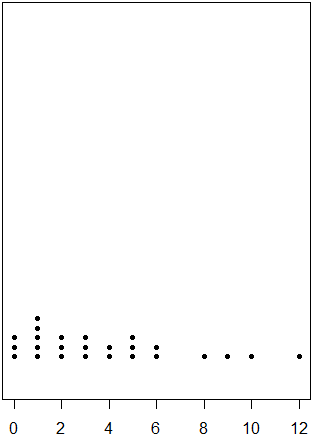
\includegraphics[trim={0 0 0 8cm}, clip]{Rplot_1}}
    \end{multicols}
    \end{mdframed}

    \paragraph*{4.}
    This is a modified version of Devore (8th ed) \S1.4: \# 45 (p.44) The article “Oxygen Consumption During Fire Suppression: Error of Heart Rate Estimation” (Ergonomics, 1991: 1469-1474) reported the following data on oxygen consumption (mL/kg/min) for a sample of ten firefighters performing a fire-suppression simulation:

    29.5, 49.3, 30.6, 28.2, 28.0, 26.3, 33.9, 29.4, 23.5, 31.6

    \paragraph*{(a)}
    Find the sample range

    \begin{mdframed}
        The sample range is $49.3 - 23.5 = \boxed{25.8}$
    \end{mdframed}

    \paragraph*{(b)}
    Find the sample variance $s^2$ from the definition (i.e., by first computing deviations, then squaring them, etc.)

    \begin{mdframed}
        \begin{equation*}
            \begin{gathered}
                S^2 = \frac{1}{n-1}\sum_{i=1}^{n}(x_{i}-\overline{x})^2 \\
                \overline{x} = \frac{1}{n}\sum_{i=1}^{n}x_i = 31.03 \\
                S^2 = \frac{1}{10-1}\sum_{i=1}^{n}(x_{i}-31.03)^2 = \frac{1}{9}((23.5 - 31.03)^2 + \dots + (49.3 - 31.03)^2) \\
                \approx \boxed{49.31}
            \end{gathered}
        \end{equation*}
    \end{mdframed}

    \paragraph*{(c)}
    Find the sample standard deviation

    \begin{mdframed}
        \begin{equation*}
            \begin{gathered}
                \sigma = \sqrt{\frac{\sum\limits_{i=1}^{n}(x_i-\overline{x})^2}{N-1}} \\
                \sum_{i=1}^{n}(x_i-\overline{x})^2 = 49.31 = S^2; \quad N = 10 \\
                \sigma = \sqrt{\frac{S^2}{N-1}} = \sqrt{\frac{49.31}{10-1}} = \boxed{5.48}
            \end{gathered}
        \end{equation*}
    \end{mdframed}

    \paragraph*{(d)}
    Find $s^2$ using the shortcut method. (Your answer should match part (b).)
    
    \begin{mdframed}
        \begin{equation*}
            \begin{gathered}
                S^2 = \frac{1}{n-1}\left[\left(\sum_{i=1}^{n}x_{i}^{2}\right)-n\overline{x}^{2}\right] \quad \text{where} \quad \overline{x}=31.03, n = 10 \\
                \sum_{i=1}^{n}x_{i}^{2} = (29.5^2 + 49.3^2 + \dots + 23.5^2 + 31.6^2) = 10,072.41   \\
                S^2 = \frac{1}{9}\left(10,072.41 - 10(31.03)^2\right) = \frac{1}{}\left(10,072.41 - \right)  = \frac{443.801}{9} \approx \boxed{49.31}
            \end{gathered}
        \end{equation*}
    \end{mdframed}

    \paragraph*{(e)}
    By how much could the observation 23.5 be increased without affecting the value of the sample median? Explain.
    
    \begin{mdframed}
        Yeah okay
    \end{mdframed}

    \paragraph*{(f)}
    Create a box plot for these data.

    \begin{mdframed}
        Yeah okay
    \end{mdframed}

    \paragraph*{5.}
    Devore \S1.4 \# 50, modified. In 1997 a woman sued a computer keyboard manufacturer, charging that her repetitive stress injuries were caused by the keyboard (Genessy v. Digital Equipment Corp.). The injury awarded about \$3.5 million for pain and suffering, but the court then set aside that award as being unreasonable compensation. In making this determination, the court identified a “normative” group of 27 similar cases and specified a reasonable award as one within two standard deviations of the mean of the awards in the 27 cases. The 27 awards were (in \$1000s) 
    
    37, 60, 75, 115, 135, 140, 149, 150, 238, 290, 340, 410, 600, 750, 750, 750, 1050, 1100, 1139, 1150, 1200, 1200, 1250, 1576, 1700, 1825, 2000

    Here is summary information:

    $\sum x_i = 20,179$ and $\sum x_{i}^{2} = 24,657,511$

    What is the maximum possible amount that could be awarded under the two-standard deviation rule?

    \begin{mdframed}
        Yeah okay
    \end{mdframed}
\end{document}